%%%%%%%%%%%%%%%%%%%%%%%%%%%%%%%%%%%%%%%%%%%%%%%%%%%%%%%%%%%%%%%%%%%%%%%%

%%% LaTeX Template for AAMAS-2025 (based on sample-sigconf.tex)
%%% Prepared by the AAMAS-2025 Program Chairs based on the version from AAMAS-2025. 

%%%%%%%%%%%%%%%%%%%%%%%%%%%%%%%%%%%%%%%%%%%%%%%%%%%%%%%%%%%%%%%%%%%%%%%%

%%% Start your document with the \documentclass command.


%%% == IMPORTANT ==
%%% Use the first variant below for the final paper (including auithor information).
%%% Use the second variant below to anonymize your submission (no authoir information shown).
%%% For further information on anonymity and double-blind reviewing, 
%%% please consult the call for paper information
%%% https://aamas2025.org/index.php/conference/calls/submission-instructions-main-technical-track/

%%%% For anonymized submission, use this
\documentclass[sigconf,anonymous]{aamas} 

%%%% For camera-ready, use this
%\documentclass[sigconf]{aamas} 


%%% Load required packages here (note that many are included already).

% \usepackage{balance} % for balancing columns on the final page
\usepackage{balance} % for balancing columns on the final page
% new package
\usepackage{algorithm}
% \usepackage{algorithmic}
\usepackage{algpseudocode}
\usepackage{amsmath}
% \usepackage[linesnumbered,ruled,vlined]{algorithm2e}
\usepackage{graphicx}
\usepackage{subfigure}
\usepackage{url}
%%%%%%%%%%%%%%%%%%%%%%%%%%%%%%%%%%%%%%%%%%%%%%%%%%%%%%%%%%%%%%%%%%%%%%%%

%%% AAMAS-2025 copyright block (do not change!)

\setcopyright{ifaamas}
\acmConference[AAMAS '25]{Proc.\@ of the 24th International Conference
on Autonomous Agents and Multiagent Systems (AAMAS 2025)}{May 19 -- 23, 2025}
{Detroit, Michigan, USA}{A.~El~Fallah~Seghrouchni, Y.~Vorobeychik, S.~Das, A.~Nowe (eds.)}
\copyrightyear{2025}
\acmYear{2025}
\acmDOI{}
\acmPrice{}
\acmISBN{}


%%%%%%%%%%%%%%%%%%%%%%%%%%%%%%%%%%%%%%%%%%%%%%%%%%%%%%%%%%%%%%%%%%%%%%%%

%%% == IMPORTANT ==
%%% Use this command to specify your EasyChair submission number.
%%% In anonymous mode, it will be printed on the first page.

\acmSubmissionID{<<EasyChair submission id>>}

%%% Use this command to specify the title of your paper.

\title[AAMAS-2025 Formatting Instructions]
{Appendix}

%%% Provide names, affiliations, and email addresses for all authors.

% \author{Arthur Pendragon}
% \affiliation{
%   \institution{Camelot Castle}
%   \city{Camelot}
%   \country{United Kingdom}}
% \email{king.arthur@camelot.uk}

% \author{Nimue}
% \affiliation{
%   \institution{The Lady's Lake}
%   \city{Avalon}
%   \country{United Kingdom}}
% \email{lady.of.the.lake@avalon.uk}

%%% Use this environment to specify a short abstract for your paper.

% \begin{abstract}
% This document outlines the formatting instructions for submissions to
% AAMAS-2025. You can use its source file as a template when writing 
% your own paper. It is based on the file `\texttt{sample-sigconf.tex}'
% distributed with the ACM article template for \LaTeX\@.
% \end{abstract}

%%% The code below was generated by the tool at http://dl.acm.org/ccs.cfm.
%%% Please replace this example with code appropriate for your own paper.


%%% Use this command to specify a few keywords describing your work.
%%% Keywords should be separated by commas.

% \keywords{Legends, Myths, Folktales}

%%%%%%%%%%%%%%%%%%%%%%%%%%%%%%%%%%%%%%%%%%%%%%%%%%%%%%%%%%%%%%%%%%%%%%%%

%%% Include any author-defined commands here.
         
\newcommand{\BibTeX}{\rm B\kern-.05em{\sc i\kern-.025em b}\kern-.08em\TeX}

%%%%%%%%%%%%%%%%%%%%%%%%%%%%%%%%%%%%%%%%%%%%%%%%%%%%%%%%%%%%%%%%%%%%%%%%

\begin{document}

%%% The following commands remove the headers in your paper. For final 
%%% papers, these will be inserted during the pagination process.

\pagestyle{fancy}
\fancyhead{}

%%% The next command prints the information defined in the preamble.

\maketitle 

%%%%%%%%%%%%%%%%%%%%%%%%%%%%%%%%%%%%%%%%%%%%%%%%%%%%%%%%%%%%%%%%%%%%%%%%

\section{Cost of schedule}
In this section,
we will proof the cost of the schedule of multiple tasks in detail.
\label{sec:cost}

\begin{figure}[htbp]
    \centering
    \subfigure[$S^1_{i,j}$]{
      \label{fig:schedule1}
      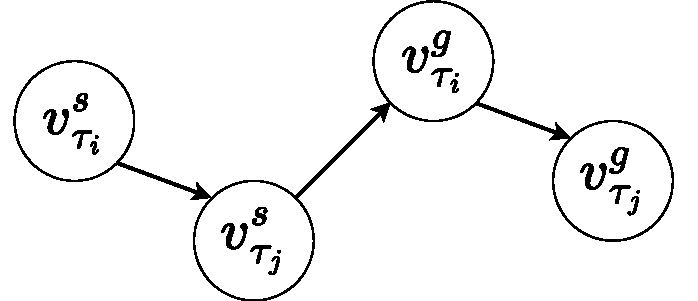
\includegraphics[width=0.4\linewidth]{Fig/path1.pdf}}
    \subfigure[$S^2_{i,j}$]{
      \label{fig:schedule2}
      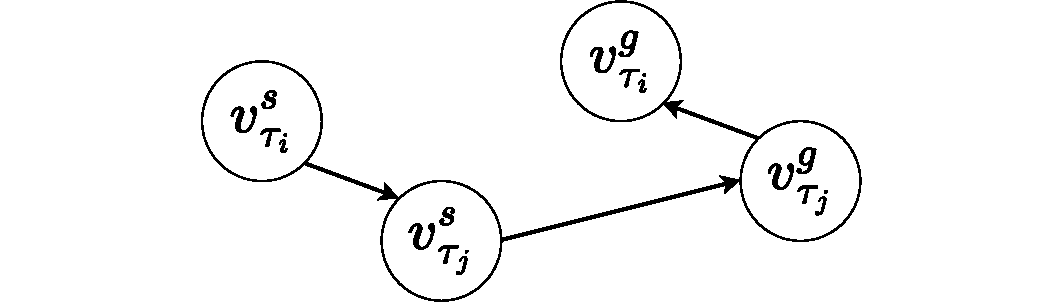
\includegraphics[width=0.4\linewidth]{Fig/path3.pdf}}
    \subfigure[$S^3_{i,j}$]{
      \label{fig:schedule3}
      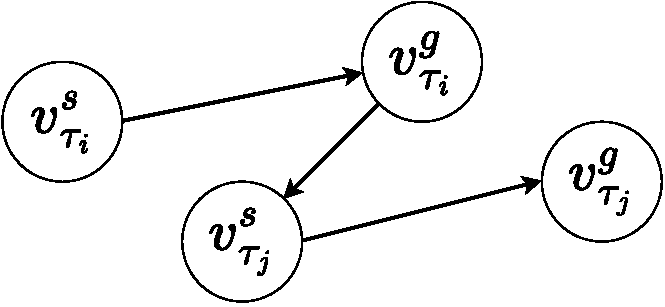
\includegraphics[width=0.4\linewidth]{Fig/path2.pdf}}
    \subfigure[$S^4_{i,j}$]{
      \label{fig:schedule4}
      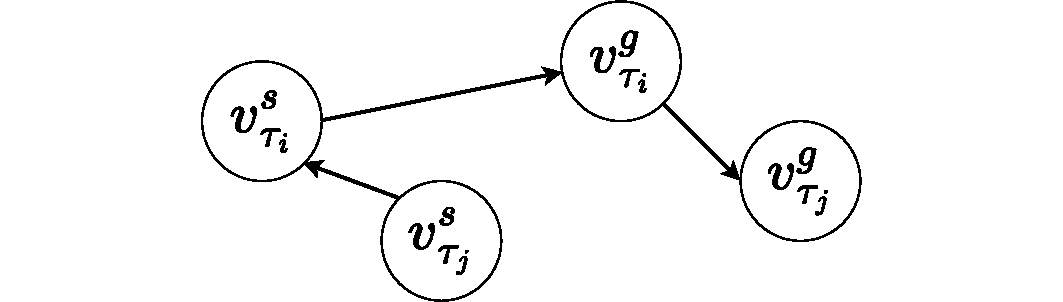
\includegraphics[width=0.4\linewidth]{Fig/path4.pdf}}
    \subfigure[$S^5_{i,j}$]{
      \label{fig:schedule5}
      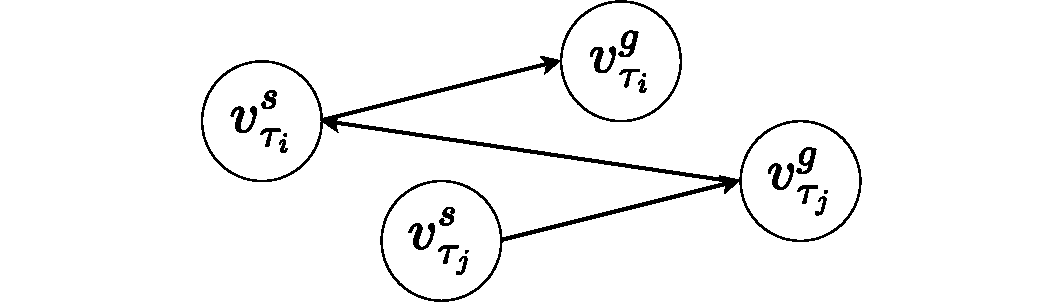
\includegraphics[width=0.4\linewidth]{Fig/path5.pdf}}
    \subfigure[$S^6_{i,j}$]{
      \label{fig:schedule6}
      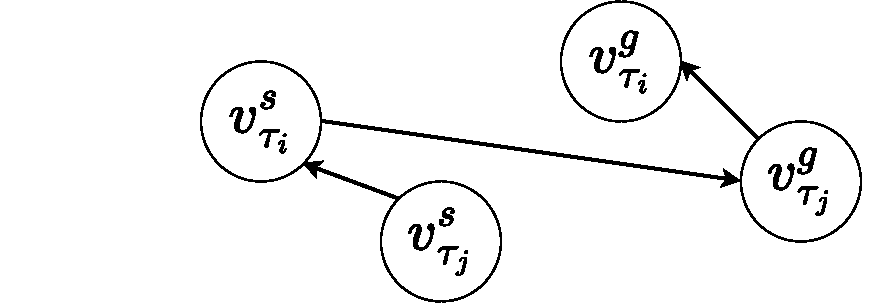
\includegraphics[width=0.4\linewidth]{Fig/path6.pdf}}
    \caption{All possible schedules of two tasks}
    \label{fig:2TP}
    \Description{All possible schedules of two tasks}
\end{figure}

As shown in Figure~\ref{fig:2TP}, there are six possible schedules for two tasks.
It means the shortest path between two tasks is the minimum cost of these six schedules.
Then, we introduce the carpooling scores between two tasks.

\begin{definition}[Carpooling Scores]
    \label{cp2}
        The carpooling scores between two tasks $\tau_{i}$ and $\tau_{j}$ is defined as 
        \begin{eqnarray}
        \label{eq:cp2}
            \delta_{\tau_{i}, \tau_{j}} = min\{Cost(S^{q}_{i,j})\} - 
            dis(v^{g}_{\tau_{i}}, v^{s}_{\tau_{i}}) - dis(v^{g}_{\tau_{j}}, v^{s}_{\tau_{j}})
            % q \in \{1, 2, 3, 4, 5, 6\}
        \end{eqnarray}
        where $q \in [1, 6] \wedge q \in \mathbb{N_+}$. $\delta_{i,j}$ is difference 
        between the best schedule of two tasks 
        and the sum of the distances between the pickup and delivery locations of the two tasks.
    \end{definition}

There exits a pickup-to-pickup path and a delivery-to-delivery path in all possible schedules of two tasks.

If the shortest schedule is $S^1_{i,j}$,
in figure~\ref{fig:schedule1},
the cost of the pickup-to-pickup path is $dis(v^{s}_{\tau_{j}}, v^{s}_{\tau_{i}})$,
and the cost of the delivery-to-delivery path is $dis(v^{g}_{\tau_{j}}, v^{g}_{\tau_{i}})$.
The cost of the schedule $S^1_{i,j}$ is $dis(v^{s}_{\tau_{j}}, v^{s}_{\tau_{i}})
+ dis(v^{g}_{\tau_{i}}, v^{s}_{\tau_{j}}) + dis(v^{g}_{\tau_{j}}, v^{g}_{\tau_{i}})$.

\begin{eqnarray}
    \label{eq:cost1}
    Cost(S^{1}_{i,j}) &=& dis(v^s_{\tau_j}, v^s_{\tau_i})+dis(v^g_{\tau_i}, v^s_{\tau_j})
      +dis(v^g_{\tau_j}, v^g_{\tau_i}) \nonumber \\
    & \geq & dis(v^s_{\tau_j}, v^s_{\tau_i})+ dis(v^g_{\tau_j}, v^s_{\tau_j}) \nonumber \\
    dis(v^g_{\tau_i}, v^s_{\tau_i})+\delta_{\tau_i, \tau_j} &\geq& dis(v^s_{\tau_j}, v^s_{\tau_i}) \label{eq:p2p1}\\
    Cost(S^{1}_{i,j}) &=& dis(v^s_{\tau_j}, v^s_{\tau_i})+dis(v^g_{\tau_i}, v^s_{\tau_j})
      +dis(v^g_{\tau_j}, v^g_{\tau_i}) \nonumber \\
    & \geq & dis(v^g_{\tau_j}, v^g_{\tau_i})+ dis(v^g_{\tau_i}, v^s_{\tau_i}) \nonumber \\
    dis(v^g_{\tau_j}, v^s_{\tau_j})+\delta_{\tau_i, \tau_j} &\geq& dis(v^g_{\tau_j}, v^g_{\tau_i}) \label{eq:d2d1}
\end{eqnarray}

If the shortest schedule is $S^2_{i,j}$,
in figure~\ref{fig:schedule2},
the cost of the pickup-to-pickup path is $dis(v^{s}_{\tau_{j}}, v^{s}_{\tau_{i}})$,
and the cost of the delivery-to-delivery path is $dis(v^{g}_{\tau_{i}}, v^{g}_{\tau_{j}})$.
The cost of the schedule $S^2_{i,j}$ is $dis(v^{s}_{\tau_{j}}, v^{s}_{\tau_{i}}) 
+ dis(v^{g}_{\tau_{j}}, v^{s}_{\tau_{j}}) + dis(v^{g}_{\tau_{i}}, v^{g}_{\tau_{j}})$.

\begin{eqnarray}
    \label{eq:cost2}
    Cost(S^{2}_{i,j}) &=& dis(v^s_{\tau_j}, v^s_{\tau_i})+dis(v^g_{\tau_j}, v^s_{\tau_j})
      +dis(v^g_{\tau_i}, v^g_{\tau_j}) \nonumber \\
    & \geq & dis(v^s_{\tau_j}, v^s_{\tau_i})+dis(v^g_{\tau_j}, v^s_{\tau_j}) \nonumber \\
    dis(v^g_{\tau_i}, v^s_{\tau_i})+\delta_{\tau_i, \tau_j} &\geq& dis(v^s_{\tau_j}, v^s_{\tau_i}) \label{eq:p2p2} \\
    Cost(S^{2}_{i,j}) &=& dis(v^s_{\tau_j}, v^s_{\tau_i})+dis(v^g_{\tau_j}, v^s_{\tau_j})
      +dis(v^g_{\tau_i}, v^g_{\tau_j}) \nonumber \\
    & \geq & dis(v^g_{\tau_i}, v^g_{\tau_j}) +dis(v^g_{\tau_j}, v^s_{\tau_j}) \nonumber \\
    dis(v^g_{\tau_i}, v^s_{\tau_i}) +\delta_{\tau_i, \tau_j} &\geq& dis(v^g_{\tau_i}, v^g_{\tau_j}) \label{eq:d2d2}
\end{eqnarray}

If the shortest schedule is $S^3_{i,j}$,
in figure~\ref{fig:schedule3},
the cost of the pickup-to-pickup path is $dis(v^{s}_{\tau_{i}}, v^{g}_{\tau_{j}}) = dis(v^g_{\tau_i}, v^s_{\tau_i}) + dis(v^s_{\tau_j}, v^g_{\tau_i})$,
and the cost of the delivery-to-delivery path is $dis(v^{g}_{\tau_{j}}, v^{s}_{\tau_{i}}) = dis(v^s_{\tau_j}, v^g_{\tau_i}) + dis(v^g_{\tau_j}, v^s_{\tau_j})$.

\begin{eqnarray}
    \label{eq:cost3}
    Cost(S^{3}_{i,j}) &=& dis(v^g_{\tau_i}, v^s_{\tau_i}) + dis(v^s_{\tau_j}, v^g_{\tau_i})
    + dis(v^g_{\tau_j}, v^s_{\tau_j}) \nonumber \\
    & = & dis(v^s_{\tau_j}, v^s_{\tau_i}) + dis(v^g_{\tau_j}, v^s_{\tau_j}) \nonumber \\
    dis(v^g_{\tau_i}, v^s_{\tau_i}) + \delta_{\tau_i, \tau_j} & = & dis(v^s_{\tau_j}, v^s_{\tau_i}) \label{eq:p2p3} \\
    Cost(S^{3}_{i,j}) &=& dis(v^g_{\tau_i}, v^s_{\tau_i}) + dis(v^s_{\tau_j}, v^g_{\tau_i})
    + dis(v^g_{\tau_j}, v^s_{\tau_j}) \nonumber \\
    & = & dis(v^g_{\tau_j}, v^g_{\tau_i}) + dis(v^g_{\tau_i}, v^s_{\tau_i}) \nonumber \\
    dis(v^g_{\tau_j}, v^s_{\tau_j}) + \delta_{\tau_i, \tau_j} & = & dis(v^g_{\tau_j}, v^g_{\tau_i}) \label{eq:d2d3}
\end{eqnarray}

$S^4_{i,j}$, $S^5_{i,j}$, and $S^6_{i,j}$ are similar to $S^2_{i,j}$, $S^3_{i,j}$, and $S^1_{i,j}$, respectively.
Because these schedules are symmetric, we can get the same results as above.

In summary,
when we observe these equations~\ref{eq:p2p1},~\ref{eq:d2d1},~\ref{eq:p2p2},~\ref{eq:d2d2},~\ref{eq:p2p3}, and~\ref{eq:d2d3},
we can draw the following two conclusions:

\begin{eqnarray}
    \label{eq:conclusion1}
    dis(v^g_{\tau_i}, v^s_{\tau_i}) + \delta_{\tau_i, \tau_j} \geq dis(v^s_{\tau_j}, v^s_{\tau_i}) \label{eq:c1} \\
    dis(v^g_{\tau_j}, v^s_{\tau_j}) + \delta_{\tau_i, \tau_j} \geq dis(v^g_{\tau_j}, v^g_{\tau_i}) \label{eq:c2}
\end{eqnarray}
where $\delta_{\tau_i, \tau_j}$ is the carpooling scores between two tasks $\tau_i$ and $\tau_j$.
Equations~\ref{eq:c1} presents the upper bound on the cost of pickup-to-pickup path of two tasks,
and equations~\ref{eq:c2} presents the upper bound on the cost of delivery-to-delivery path of two tasks.

Then, we can get the cost of the schedule of multiple tasks.
In this paper, we introduce a novel method to schedule multiple tasks.

\begin{figure}
    \centering
    \includegraphics[width=0.8\linewidth]{Fig}
    \caption{The schedule of multiple tasks}
    \label{fig:smt}
    \Description{The schedule of multiple tasks}
\end{figure}


\balance

% \begin{acks}
% If you wish to include any acknowledgments in your paper (e.g., to 
% people or funding agencies), please do so using the `\texttt{acks}' 
% environment. Note that the text of your acknowledgments will be omitted
% if you compile your document with the `\texttt{anonymous}' option.
% \end{acks}

%%%%%%%%%%%%%%%%%%%%%%%%%%%%%%%%%%%%%%%%%%%%%%%%%%%%%%%%%%%%%%%%%%%%%%%%

%%% The next two lines define, first, the bibliography style to be 
%%% applied, and, second, the bibliography file to be used.

% \bibliographystyle{ACM-Reference-Format} 
% \bibliography{sample}

%%%%%%%%%%%%%%%%%%%%%%%%%%%%%%%%%%%%%%%%%%%%%%%%%%%%%%%%%%%%%%%%%%%%%%%%

\end{document}

%%%%%%%%%%%%%%%%%%%%%%%%%%%%%%%%%%%%%%%%%%%%%%%%%%%%%%%%%%%%%%%%%%%%%%%%

